

%----------------------------------------------------------------------------------------
%	PACKAGES AND OTHER DOCUMENT CONFIGURATIONS
%----------------------------------------------------------------------------------------

\documentclass[fleqn,8pt]{SelfArx} % Document font size and equations flushed left

\usepackage[portuguese]{babel} % Specify a different language here - english by default
\usepackage{cmap}				% Mapear caracteres especiais no PDF
\usepackage{lmodern}			% Usa a fonte Latin Modern
\usepackage[T1]{fontenc}		% Selecao de codigos de fonte.
\usepackage[utf8]{inputenc}		% Codificacao do documento (conversão automática dos acentos)
\usepackage{indentfirst}		% Indenta o primeiro parágrafo de cada seção.
\usepackage{nomencl} 			% Lista de simbolos
\usepackage{color}				% Controle das cores
\usepackage{graphicx}			% Inclusão de gráficos

%Para tipos de Itens
\usepackage{amssymb}
\usepackage{pifont} 
\usepackage{bbding}
\usepackage[normalem]{ulem} % Para fazer strikeout com \sout{Texto}

\usepackage[final]{pdfpages} % Para incluir anexos no final

%\usepackage{fancyhdr}
%\usepackage{lastpage}

\newcommand{\figpath}[1] {C:/Users/Ronie/Documents/Saturno/LOCAL/EXEDADOS/FIGURAS/#1}

%Escolher um dos tipos de itens:
%\renewcommand\labelitemi{-} % Traçado Pequeno
%\renewcommand\labelitemi{--} % Traçado Médio
%\renewcommand\labelitemi{---} % Traçado Grande
%\renewcommand\labelitemi{$\star$} % Símbolo de Estrela
%\renewcommand\labelitemi{\scriptsize$\blacksquare$} % Símbolo de Quadradinho
%\renewcommand\labelitemi{\Checkmark} % Símbolo de V
%\renewcommand\labelitemi{\XSolidBrush} % Símbolo de X
%\renewcommand\labelitemi{\ding{51}} % Outro Símbolo de V
%\renewcommand\labelitemi{\ding{55}} % Outro Símbolo de X
%\renewcommand\labelitemi{\tiny$\bullet$} % Símbolo de Bolinha

\renewcommand\labelitemi{\tiny$\bullet$} % Símbolo de Bolinha
\renewcommand\labelitemii{--} % Símbolo de Traço Médio

%----------------------------------------------------------------------------------------
%	COLUMNS
%----------------------------------------------------------------------------------------

\setlength{\columnsep}{0.20cm} % Distance between the two columns of text
\setlength{\fboxrule}{0.75pt} % Width of the border around the abstract

%----------------------------------------------------------------------------------------
%	COLORS
%----------------------------------------------------------------------------------------

\definecolor{color1}{RGB}{0,0,90} % Color of the article title and sections
\definecolor{color2}{RGB}{0,20,20} % Color of the boxes behind the abstract and headings

%----------------------------------------------------------------------------------------
%	HYPERLINKS
%----------------------------------------------------------------------------------------

\usepackage{hyperref} % Required for hyperlinks
\hypersetup{hidelinks,colorlinks,breaklinks=true,urlcolor=color2,citecolor=color1,linkcolor=color1,bookmarksopen=false,pdftitle={Title},pdfauthor={Author}}

%----------------------------------------------------------------------------------------
%	ARTICLE INFORMATION
%----------------------------------------------------------------------------------------

\JournalInfo{Projeto DNC} % Journal information
\Archive{Documentação} % Additional notes (e.g. copyright, DOI, review/research article)

\PaperTitle{Projeto DNC} % Article title

\Authors{rppsys@gmail.com} % Authors
\Authors{Ronie Paulucio Porfirio} % Authors
\affiliation{} % Author affiliation
\affiliation{} % Author affiliation
\affiliation{} % Corresponding author

\Keywords{} % Keywords - if you don't want any simply remove all the text between the curly brackets
\newcommand{\keywordname}{Palavras-chave} % Defines the keywords heading name

%----------------------------------------------------------------------------------------
%	ABSTRACT
%----------------------------------------------------------------------------------------

\Abstract{Projeto Dança é uma forma de tentar escrever os passos de uma dança em par de forma a não esquecer.}

%----------------------------------------------------------------------------------------

\begin{document}
\flushbottom % Makes all text pages the same height
\maketitle % Print the title and abstract box
\tableofcontents % Print the contents section
\thispagestyle{empty} % Removes page numbering from the first page

%----------------------------------------------------------------------------------------
%	ARTICLE CONTENTS
%----------------------------------------------------------------------------------------



\section{Atenção: Isto é um RASCUNHO da documentação do projeto}

Esse documento é um esboço da documentação do projeto.

Estou desenvolvendo isso como um projeto hobby no pouco tempo livre que tenho, dessa forma, essa documentação estará repleta de erros de portugues, abreviaturas e observações. Além de seções onde eu já pulo de cara para alguma lista de coisas que achei importante registrar logo antes que as idéias se perdessem. Um documento final teria que passar muitas revisões antes de se tornar publicável.

\section{Introdução}


Este documento ainda é apenas um esboço.

Existem pelo menos três formas de dança: individual, em par e em grupo.

Nas danças em par, geralmente, um condutor conduz os movimentos do conduzido. Na cultura tradicional geralmente o condutor é o homem e o conduzido é a mulher. 

Uma das maiores dificuldades enfrentadas é que não existe um sistema simples de representação dos passos de dança acessível à população.

Existe o Syllabus e outras notações de coreografia, mas todos são sistemas muito técnicos e muito complexos.

Em danças em par, por exemplo, o recurso mais utilizado para tentar gravar uma sequencia de passos de dança é o vídeo em que se filmam um par de dançarinos executando os passos da sequencia.

O objetivo é desenvolver um sistema universal, simples, intuitivo de descrição de passos de dança em par de forma que os passos possam ser escritos, armazenados e, posteriormente, reproduzidos.


\subsection{Definições}


\subsubsection{Passo Fundamental}

Passo fundamental é um passo. É o movimento de passo na qual um e apenas um pé se desloca enquanto o outro permanece fixo. O passo pode ser dar de duas formas:

\begin{itemize}
	\item \textbf{passo completo ou passo simples ou simplesmente passo}: Um passo completo é aquele que finaliza com a transferência do peso do corpo para o conjunto perna-pé que deu o passo. O próximo passo que será dado deve ocorrer obrigatoriamente com o pé que permaneceu fixo durante o movimento deste.
	
	\item \textbf{passo para marcação}: Um passo para marcação ou apenas marcação é um passo que não se completa. Ele apenas marca em algum lugar, mas o peso do corpo não é transferido para o mesmo. Dessa forma, o próximo passo que será dado vai ocorrer obrigatoriamente com o mesmo pé que acabou de ser usado para fazer essa marcação. Nas danças em pares, essa marcação pode ser feita apenas tocando algum elemento do pé (ponta ou calcanhar) no chão, mas sem transferir o peso. Nesta linguagem, passos-marcação serão identificados pela presença de um asterisco (*) no código do passo fundamental.
		
\end{itemize}


\subsubsection{Movimento Intermediário ou Caminho}


Um movimento intermediário é uma sequência de passos fundamentais. Por esse motivo, também será chamado de caminho. Um caminho geralmente ocorre dentro de uma unidade de marcação da música. 

Geralmente um caminho começa de um estado inicial e termina em um estado final. E aí será necessário um outro caminho para sair desse estado final e voltar para o primeiro estado inicial. 

Observações:

\begin{itemize}
	\item caminho oposto: Um caminho é oposto a outro caminho quando um desfaz o o que o outro fez no mesmo tempo. O editor de caminhos deveria ser capaz de identificar caminhos opostos. 
\end{itemize}

\subsubsection{Movimento de Dança ou Sequência}

Um movimento de dança é uma sequência de movimentos intermediários ou uma sequencia de caminhos. Nesse trabalho, chamaremos os movimentos de dança com o nome simples de sequencia.


\subsection{Objetivo}

O objetivo é desenvolver uma linguagem de descrição de movimentos de dança em par universal, legível, fácil de ler, entender e escrever. Embora o maior desafio seja descrever as sequencias de  passos, também chamadas de footwork, ou trabalho dos pés, essa linguagem também deve descrever os demais elementos que compõe o movimento como a posição relativa do casal, os estados das mãos e até movimentos de tronco, quadril, pescoço, etc.

Como objetivo secundário, desenvolver ferramentas em linguagem computacional para criar as sequências de movimentos. Um editor de caminhos e um editor de sequências.

É como se eu estivesse desenvolvendo uma linguagem de programação para programar uma sequência de movimentos de dança em par.

Um terceiro e último objetivo, é criar um compilador ou interpretador capaz de ler o programa e interpreta-lo. Qual a saída? Uma dança. Dessa forma, o interpretador é um software capaz de gerar um personagem digital 3D que vai executar os passos de dança na ordem que eles aparecem no programa. 

E assim teremos um sistema completo para escrever sequências de dança e ver os personagens digitais executando esses movimentos.




 




\section{Sistema de Orientação}

O sistema de orientação é relativo a quem realiza o movimento. Esse sistema relativo é muito melhor do que o sistema absoluto pois permite que sejam objervados as simetrias da dança.


\subsection{Sentidos de Giros}


Dentro Direita

Dentro Esquerda

Fora Direita

Fora Esquerda

Ver tabela ODS



\section{Classe Mão}


A mão é uma classe parecida com a pé.

\subsection{Objetos}

Terá os objetos:

\begin{itemize}
	\item mE = Mão esquerda do agente
	\item mD = Mão direita do agente
	\item mM = Ambas as mãos do agente 
\end{itemize}

As diferença para a classe pé, é que a classe mão possui o objeto mM que serve para aplicar métodos para as duas mãos ao mesmo tempo.

\subsection{Estados}

As mãos podem assumir diversos estados. Estados são descrições estáticas das posições. Ver tabela ODS para as posições.

Os estados podem ser Frente, Costas, Dog, Cat, Esquerda do Condutor com Direita do Conduzido (somente E), Direita (idem anterior), Esquerda com Esquerda (EE) ou Esquerda Invertida, Direita com Direita (DD) ou Direita Invertida.

\subsection{Métodos}

Assim como os pé possuem métodos, as mão também possuem. 


Para os pés os métodos adotam como referencial o pé que realiza o movimento em relação ao pé que fica parado.
pD.ABR manda vc abrir o pé direito em relação ao pé esquerdo que fica parado. 

Contudo, nas mãos, podemos movimentar a mão esquerda e a mão direita ao mesmo tempo em uma infinidade de movimentos de condução no espaço 3D.
O objetivo desse projeto é representar os movimentos de dança de forma simplificada se forma que os passos possam ser reproduzidos a partir
da leitura de um texto ou pelo menos lembrados.

Então eu preciso estudar os métodos das mãos.

Eu já filosofei e cheguei a conclusao que novamente os movimentos mais básicos ocorrem com o referencial da mão que 
realiza o movimento.

Movimentos

\begin{itemize}
	\item Puxar
	\item Empurrar
\end{itemize}

Mesmo assim vc pode puxar ou empurrar no plano xy para fazer condução, ou em planos xyz.

Por enquanto vou me preocupar apenas com o plano xy. Movimentos no eixo Z fica para o futuro.



\textbf{Movimentos Esquerda (ED) apenas ou Direita (DE) Apenas}

\begin{itemize}
	\item Mover para Dentro
	\item Mover para Fora
	\item Empurrar para Distante
	\item Puxar para próximo
	\item Girar para Fora 
	\item Girar para Dentro
\end{itemize}



\textbf{Movimentos com as duas mãos dadas:}

Os movimentos com as duas mãos dadas mM são mais complicados pois mover para dentro com a mão direita possui sentido de movimento
oposto a mover para dentro com a mao esquerda. 

Uma forma de tratar isso é adotando os sentidos esquerda e direita. 

Assim: 

\begin{itemize}
	\item Mover para a direita
	\item Mover para a esquerda
	\item Empurrar para Distante
	\item Puxar para próximo
\end{itemize}


Outra é adotando uma das mãos como o referencial para movimentos com as duas mãos dadas. 
E ai, podemos usar os mesmos movimentos que para mãos soltas.

Dessa forma, vou adotar o BRAÇO DIREITO como o braço referencial para movimentos de braços dados mM:

E assim temos:

\begin{itemize}
	\item Mover para Dentro - Vai para a esquerda
	\item Mover para Fora - vai para a direita 
	\item Empurrar para Distante
	\item Puxar para próximo
	\item Girar para Fora 
	\item Girar para Dentro
\end{itemize}


Uma última definição é com relação ao giro. Enquanto o movimento adota como referencial a mão do condutor.
O referencial do giro é o conduzido.

Assim Girar para Fora é para fora no referencial do conduzido. Essa definição facilita o entendimento.

mM.girar para dentro = realiza um movimento de  giro para fora do condutor mas para dentro do conduzido.

mM adota o mesmo referencial do mD logo 

mD.girar para dentro, o giro ocorre para dentro do condutor e do conduzido. E ai o conduzido dá um giro Dentro Esquerdo.

Preciso melhorar mais isso até ficar simples e intuitivo.









\section{criarDBTemp}

O arquivo criarDBTemp.py cria os bancos de dados para cada ritmo.

\subsection{Descrição das Tabelas}

O banco de dados é estruturado em forma de um grafo orientado. Para isso são importantes 2 tabelas: 

\begin{enumerate}
	\item \textbf{tbNO} - A tabela tbNO contém os nós do grafo. 
	\item \textbf{tbAD} - A tabela tbAD contém as ligações entres os nós.	
\end{enumerate}

Além dessas duas tabelas, podem existir diversas outras tabelas de tipos de nós. Essas tabelas contem as informações de cada nó do grafo. Contudo, neste banco de dados genérico criarDBTemp só existe até o momento uma única tabela de informações: A tabela tbSTP.

\begin{enumerate}
	\item \textbf{tbSTP} - A tabela tbSTP contém as informações da estrutura organizacional dos passos desse ritmo.
\end{enumerate}

A seguir, detalha-se cada uma dessas estruturas.


\subsubsection{Tabela tbNO}

tbNO é a tabela com os Nós do grafo orientado.

Essa tabela possui a seguinte estrutura:

\begin{itemize}
	% -------------------------------------------------------------------------------
	\item \textbf{cod}: Inteiro - Código numérico único do nó.
			\begin{itemize}
				\item a
			\end{itemize}

	% -------------------------------------------------------------------------------
	\item \textbf{typeNO}: String - Tipo de nó. Indica para qual tabela aponta o nó.
			\begin{itemize}
				\item root: Não aponta para nenhuma tabela, este é o nó ROOT. Ele aponta para todas as estruturas do banco.
				\item stp: Indica que o nó aponta para um registro da tabela tbStp.
			\end{itemize}
	% -------------------------------------------------------------------------------	
	\item \textbf{codPointer}: Inteiro - Código do registro na tabela typeNO para o qual esse nó aponta.
			\begin{itemize}
				\item a
			\end{itemize}
	% -------------------------------------------------------------------------------	
	\item \textbf{drwGX}: Informações para desenhar o nó na tela.
			\begin{itemize}
				\item a
			\end{itemize}
	% -------------------------------------------------------------------------------	
	\item \textbf{drwGY}: Informações para desenhar o nó na tela.
			\begin{itemize}
				\item a
			\end{itemize}
	% -------------------------------------------------------------------------------	
	\item \textbf{drwLev}: Informações para desenhar o nó na tela.
			\begin{itemize}
				\item a
			\end{itemize}
	% -------------------------------------------------------------------------------	
	\item \textbf{drwHei}: Informações para desenhar o nó na tela.
			\begin{itemize}
				\item a
			\end{itemize}
	% -------------------------------------------------------------------------------	
	\item \textbf{drwPos}: Informações para desenhar o nó na tela.
			\begin{itemize}
				\item a
			\end{itemize}
	% -------------------------------------------------------------------------------	
	\item \textbf{drwRel}: Informações para desenhar o nó na tela.
			\begin{itemize}
				\item a
			\end{itemize}
	% -------------------------------------------------------------------------------	
	\item \textbf{booActive}: Indica se o nó está ativo. Ainda não estou usando isso para nada.
			\begin{itemize}
				\item 1 = Ativo
				\item 0 = Inativo
			\end{itemize}
	% -------------------------------------------------------------------------------	
	
\end{itemize}

% ########################################################################

\subsubsection{Tabela tbAD}

tbAD é a tabela que indica que nó se liga a qual outro nó e o tipo de ligação.

A filosofia adotada é que uma ligação DE PARA é unidirecional.

Essa tabela possui a seguinte estrutura:

\begin{itemize}
	% -------------------------------------------------------------------------------
	\item \textbf{cod}: Inteiro - Código numérico único do registro que indica uma ligação.
			\begin{itemize}
				\item a
			\end{itemize}

	% -------------------------------------------------------------------------------
	\item \textbf{typeAD}: String - Tipo de ligação.


\emph{Atualmente estou descrevendo os tipos de cada tbSTP, mas não é isso que farei pois é redundante. Criarei novos tipos de ligação.}

Os typeAD possuem a seguinte formação: D.nome

\begin{itemize}
	\item D : Número que indica a direção. 1 indica que é uma ligação que cria uma árvore ordenada. 2 indica que é uma ligação entre nós da árvore e, portanto, não vou seguir. 1 também indica que é uma ligação unidirecional. 2 - indica que a ligação é bidirecional, então,
	
	\item nome: É o nome da ligação.
	
\end{itemize}


Os tipos de ligação podem ser:


			\begin{itemize}
				\item \textbf{1.org}: Ligação gerada pelo arquivo csv escrita pelo usuário para ORGANIZAR os passos de dança.
				\item \textbf{1.prop}: Ligação gerada pelo \emph{VERIFICADOR} para criar propriedades.

				\item \textbf{2.vv}: Acrônimo para vai-vem - Ligação manual entre duas leafs indicando que PARA UM MESMO AGENTE (condutor ou conduzido) o que uma sequencia de passos faz a outra volta para o mesmo lugar de partida. 
				
				Ex.: Se o passo condutor.base.hoz.esq vai para a esquerda, então o passo condutor.base.hor.dir volta para a posição inicial. Então esses dois passos serão ligados por uma conexão \textbf{vv}. 
				
				Pela filosofia de unidirecionalidade do tbAD, passos conectados pela conexão do tipo \textbf{vv} deverão ter 2 registros para cada possível deslocamento.
			
				
				\item \textbf{2.par}: Indica que o passo de um agente é um possível par para o outro agente. 
				
				Ex.: No forró o passo \emph{condutor.base.ver.frt} faz par com o passo \emph{conduzido.base.ver.trs} e vice versa. 
				
				Como a filosofia adotado é que todo registro da tabela AD é sempre unidirecional, preciso criar sempre dois tbADs um para conectar a IDA e o outro a VOLTA.
			
			
			
			\end{itemize}

	% -------------------------------------------------------------------------------	
	\item \textbf{codFrom}: Código do tbNO DE onde PARTE a ligação.
	% -------------------------------------------------------------------------------	
	\item \textbf{codTo}: Código do tbNO PARA onde CHEGA a ligação.
	% -------------------------------------------------------------------------------	
	
\end{itemize}

% ########################################################################
% ####### TABELA tbSTP    ################################################
% ########################################################################



\subsubsection{Tabela tbSTP}

tbSTP é a tabela que vai formar a descrição de todos os passos (Steps) do ritmo. Ela vai organizar os passos em uma estrutura de árvore que servirá para gerar o nome dos arquivos que indicam as sequências de passos fundamentais para se dançar esse ritmo.

Essa tabela possui a seguinte estrutura:

\begin{itemize}
	% -------------------------------------------------------------------------------
	\item \textbf{cod}: Inteiro - Código numérico único do nó.
	% -------------------------------------------------------------------------------
	\item \textbf{strNAME}: String - Nome.
	% -------------------------------------------------------------------------------	
	\item \textbf{strTYPE}: String - Tipo de Nó. Esses tipos são fornecidos pelo arquivo csv, mas são tipos definidos (não pode ser qualquer coisa) seguem uma regra.
	
	Os tipos de nós possíveis são:
	
	\begin{itemize}
		\item \textbf{root}: indica o nó root.
		\item \textbf{mod}: Modalidade do ritmo. Ex.: Zouk, Forró, Sertanejo.
		\item \textbf{sub}: Submodalidade do ritmo. Ex.: Brasileiro, Versão 1, V1.
		\item \textbf{cond}: Indica se trata-se de um passo pertencente ao Condutor ou Conduzido.
		\item \textbf{tag}: Tag indica que este é um nó que faz parte de uma hierarquia de classificação do passo. Não é o passo propriamente dito ainda. É uma forma de organizar os passos. Uma tag pode se ligar a outras tags até finalmente chegarmos na folha leaf que é o último elemento da árvore gerada por ligações 1.org. 
		\item \textbf{leaf}: Elemento folha do passo. Este é o nome que diferencia um passo entre seus irmãos dentro de uma mesma tag de classificação. Veja que o nome do passo todo sai do elemento ROOT e vai até o elemento LEAF usando underlines para se gerar o nome do arquivo .txt (que no futuro vou dar a extensão .stp) que contem a sequencia de passos fundamentais. São os leafs que podem ser ligados entre sí por outras ligações como 2.vv e 2.par para indicar pares de passos vai-e-vem e pares de passos condutor-conduzido respectivamente.
		\item \textbf{prop}: Indica que o nó é uma propriedade gerada pelo VERIFICADOR. As propriedades são nós gerados pela ligação 1.prop
	\end{itemize}


\item \textbf{strVALUE}: String - Cada  nó pode carregar também um valor. É o caso dos nós do tipo prop que vão armazenar valores. Nos nós de classificação o valor do strVALUE é string vazia.

\item \textbf{codNO}: Inteiro - Aponta para o registro da tabela tbNO que, por sua vez aponta para o meu código pela propriedade codPointer. Ficou redundante mas é para facilitar a programação. Posso sair da tabela tbNO e encontrar o registro tbSTP para o qual ele aponta ou sair do tbSTP e chegar no registro tbNO que aponta para mim.

	
\end{itemize}

% ########################################################################
% ########################################################################
% ########################################################################


\section{criarDBTree}

O arquivo criarDBTree.py cria o banco de dados com os passos mais fundamentais.

Destalhes do banco ficam para depois.


\section{Passos Fundamentais}

\subsection{Modificadores de Passos}


Os modificadores de translação e rotação são declarados dentro de parenteses.

Podem ser:

\begin{itemize}
	\item \textbf{rot} - Modificador de Rotação
	\item \textbf{tra} - Modificador de Translação
\end{itemize}

\subsection{Modificadores de Rotação rot}


O modificador de rotação leva duas letras. A primeira indica o sentido e a segunda o giro.

\subsubsection{Primeira Letra - Sentido}

Sentidos:

\begin{itemize}
	\item \textbf{f} - Sentido para fora.
	\item \textbf{d} - Sentido para dentro.
\end{itemize}


Ver as figuras com as definições do que é para fora e o que é para dentro. 

Macete: Quando o braço abraça levando a palma da mão com os polegares para cima em direção ao peito o sentido é dentro. Sempre. Mesmo de costas.

Quando o braço se movimenta na direção da palma da mão com o polegares para baixo em direção a bater nas costas é fora. Sempre.


\subsubsection{Segunda Letra - Ângulo de rotação}

Rotações

\begin{itemize}
	\item \textbf{q} - 90 graus
	\item \textbf{v} - 180 graus
	\item \textbf{t} - 30 graus
\end{itemize}


\subsection{Exemplo de Modificadores de Rotação}


pD.FRT(rot=fq)

Leva o pé direito para frente rotacionando para fora (sentido negativo) em 90 graus.

pD.FRT(rot=dq)

Leva o pé direito para frente rotacionando para dentro (sentido positivo) em 90 graus.


Colocar aqui todas as possibilidades e estuda-las.


Fazer uma tabela Ver projetoDNC.ods




\subsection{Modificadores de Translação Tra}


A translação pode ocorrer a partir de 8 pontos a partir da posição final do pé.


Então vc verifica qual seria a posição final do pé e a partir dali traça uma estrela de 8 pontas. Norte Sul Leste Oeste e ai teremos as possibilidades.


Faço mais depois...


























%------------------------------------------------
\phantomsection
\section*{Bons estudos} 

%----------------------------------------------------------------------------------------
%	REFERENCE LIST
%----------------------------------------------------------------------------------------
%\phantomsection
%\bibliographystyle{unsrt}
%\bibliography{sample}
%----------------------------------------------------------------------------------------


%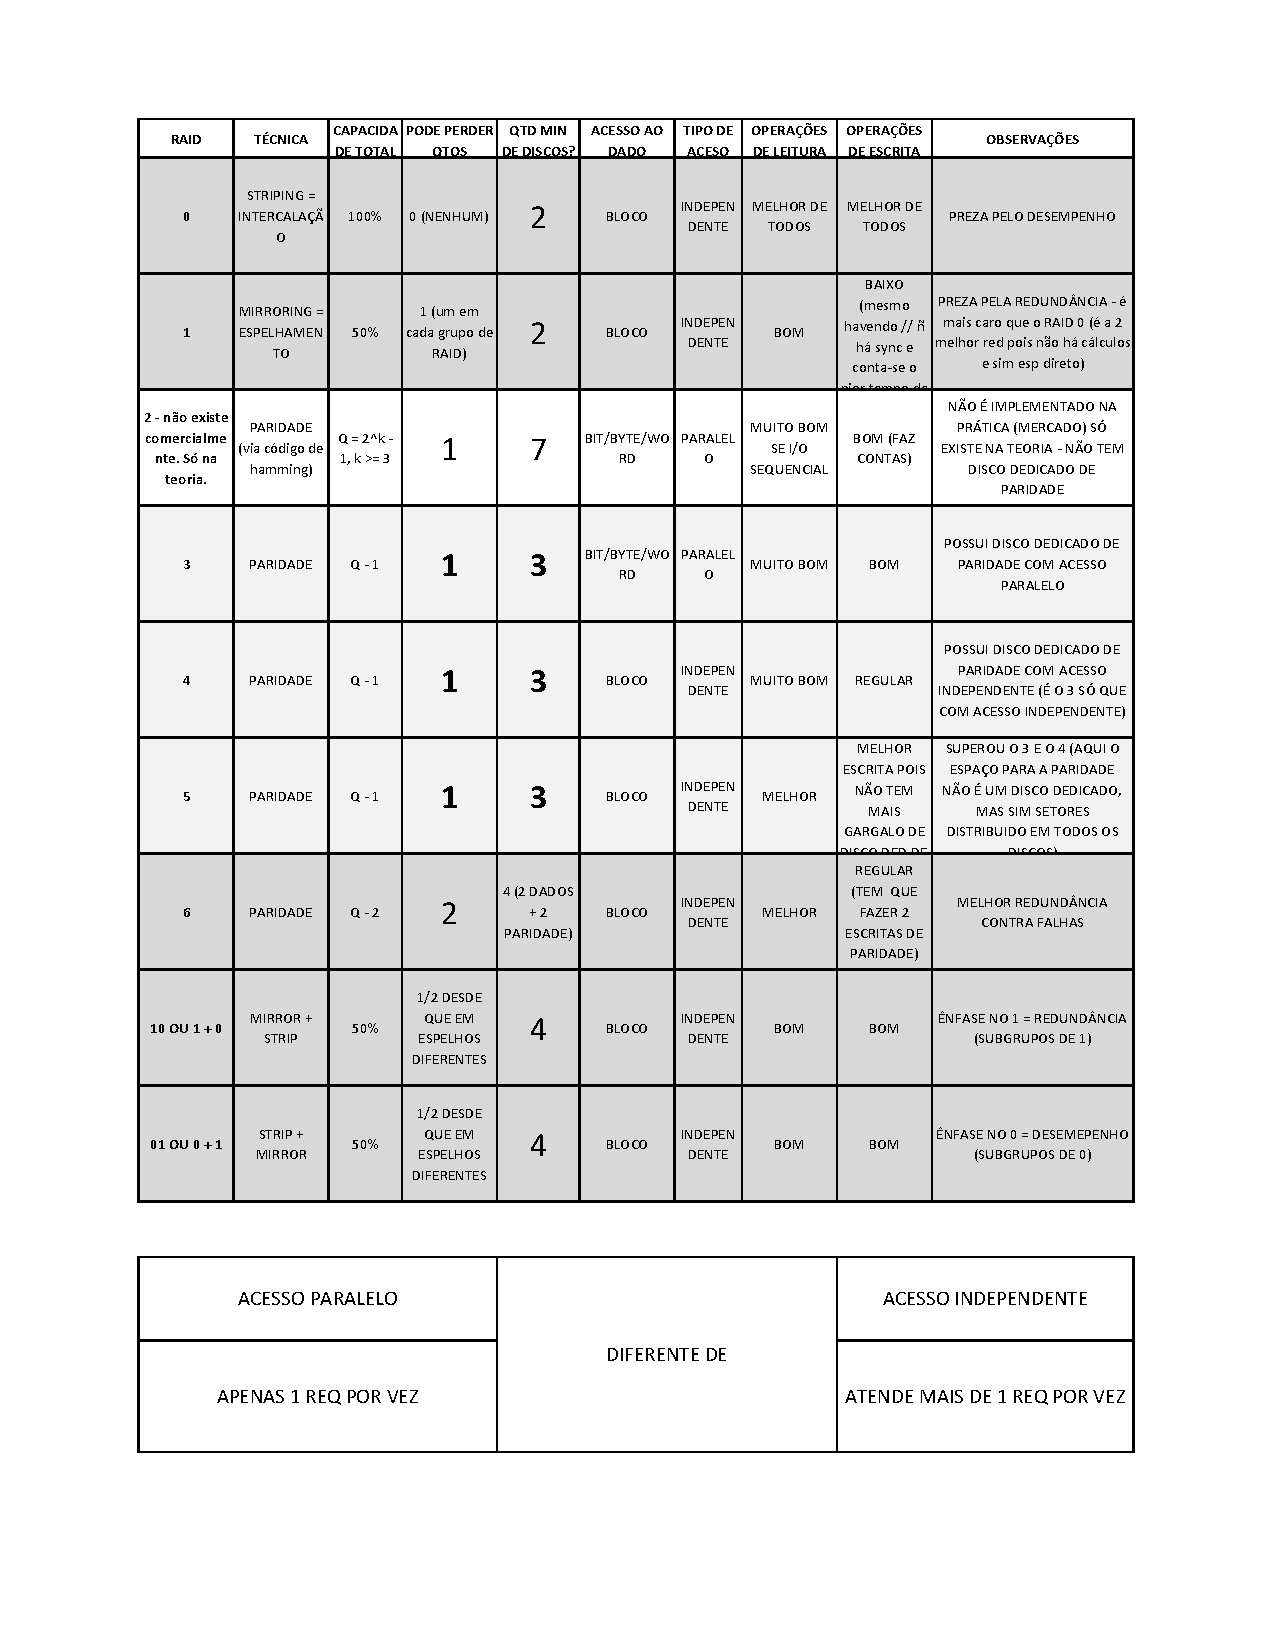
\includepdf[pages=-]{ANEXOS/RAID.pdf}
%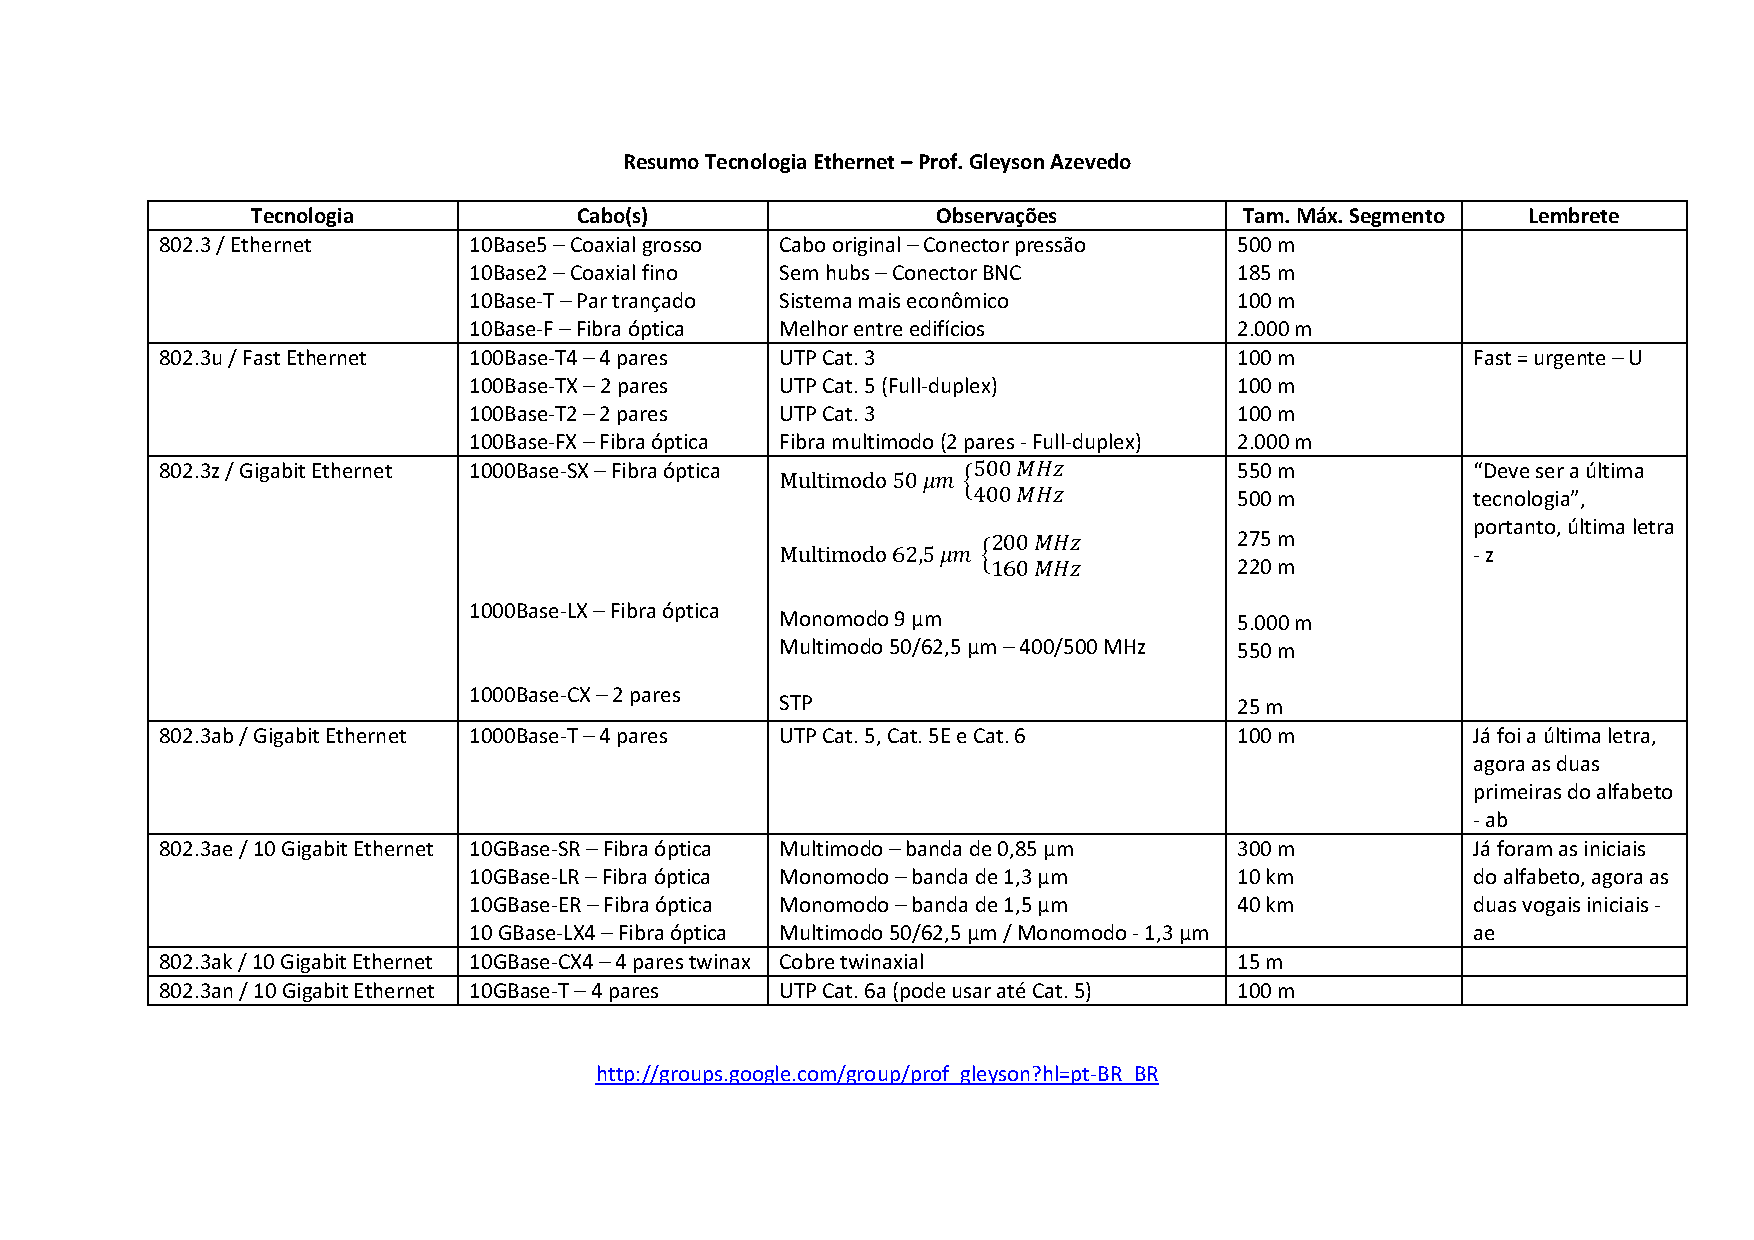
\includepdf[pages=-,angle=90]{ANEXOS/ETHERNET.pdf}



\end{document}

